\documentclass[handout]{beamer}
\usetheme{UniKlu}
\usepackage[backend=bibtex,style=numeric]{biblatex}
\usepackage[english]{babel}
\addbibresource{/media/donkarlo/Elements/projs/research/refs.bib}


\usepackage{xcolor}

\title{Toward artificial collective self-awareness}
\author{Mohammad Rahmani}
\institute{Decide Doctrol Group}

\begin{document}
\begin{frame}
	\maketitle
\end{frame}

\begin{frame}{Self-awareness (SA) - Definition}
	\begin{itemize}
		\item The capacity to become the object of one’s \textbf{own attention}, which arises when an agent focuses \textbf{not only} on the \textbf{external environment} but also on the \textbf{internal milieu} \cite{morin-2006-levels-of-consciousness-and-self-awareness-a-comparison-and-integration-of-various-neurocognitive-views}. 
	\end{itemize}
\end{frame}

\begin{frame}{SA - Definition (Literal)}
	\begin{itemize}
		\item Giving the ability to computers to program themselves in unseen circumstances.
		\item Casual-temporal inference of agents behavior on the environment and vice-versa. 
			\begin{itemize}
				\item If I do \textbf{x}, what will happen outside? (Part of behavioral Active awareness)
				\item If \textbf{y} happens outside, how would it affect me? (Part of behavioral Passive awareness)
			\end{itemize}
	\end{itemize}
\end{frame}

\begin{frame}{SA - Levels}
	See \cite{lewis-2017-towards-a-framework-for-the-levels-and-aspects-of-self-aware-computing-systems} - Ordered from basic to advanced
	\begin{itemize}
		\item \textbf{Ecological self} The most basic, referring the ability of an agent to react to a stimuli.
		
		\item \textbf{Interpersonal self} Awareness of external interaction such that limited adaptation to performance of basic homeostatic tasks is achieved.
		
		\item \textbf{Extended self}  Permit reflection of interactions over time. The organism is aware of the existence of past and future.
		
		\item \textbf{Private self} The agent can process more advanced information concerning itself,
		
		\item \textbf{Conceptual self}: The capability of constructing and reasoning
		about an abstract symbolic representation of itself (AI's goal).
	\end{itemize}
\end{frame}

\begin{frame}{SA - Aspects}
	See \cite{lewis-2017-towards-a-framework-for-the-levels-and-aspects-of-self-aware-computing-systems}
	\begin{itemize}
		\item \textbf{Identity Awareness}: The ability to recognize and model the identity of agents.
		\item \textbf{State Awareness}: The ability to model and recognize the states of oneself, the world or other entities within it
		\item \textbf{Time Awareness}: The knowledge of past or potential future basic stimuli
		\item \textbf{Interaction Awareness}: The ability to taking into account casual patterns of
		interactions between entities.
	\end{itemize}
\end{frame}

\begin{frame}{SA - Aspects (2)}
	See \cite{lewis-2017-towards-a-framework-for-the-levels-and-aspects-of-self-aware-computing-systems}
	\begin{itemize}
		\item \textbf{Behavior Awareness}: The ability to model the internal behavior of the system
		or behavior of external entities.
		\item \textbf{Goal Awareness}: the ability to conceptualize the internal factors that drive the behavior, such as a system’s goals, objectives, and constraints.
		\item \textbf{Belief Awareness}: Things believed to be true by a system which do \textbf{NOT} need to capture the notion of time.
		\item \textbf{Expectation Awareness}: Combines belief awareness and time awareness, to form models that express what the system or others believe about how the world will unfold over time
	\end{itemize}
\end{frame}

\begin{frame}{Why SA in AI?}
	\section{Why SA in AI?} The driving motivation for the transfer of biological SA concepts
	to artificial systems is to improve:
	\begin{itemize}
		\item autonomy
		\item robustness
		\item scalability
	\end{itemize}
	In intelligent Agents (IA).
\end{frame}

\begin{frame}{SA IA Essential requirements}
	See \cite{regazzoni-2020-multi-sensorial-generative-and-descriptive-self-awareness-models-for-autonomous-systems}
	\begin{itemize}
		\item \textbf{Initialization}: Initial knowledge from which an agent starts building its own memories (Training phase. \emph{Techniques}: Random walk, Driving an autonomous vehicle a few times human agent. etc). \textbf{Biology}: Implemented into genes.
		\item \textbf{Memorization}: Capability to store and retain information \textbf{Biology}: Brain's capability to fire group memory related neurons in case of facing familiar patterns of stimuli. 
		\item \textbf{Inference}: Ability to predict own future states \textbf{Biology}: See "Predictive coding theory" in \cite{seth-2013-interoceptive-inference-emotion-and-the-embodied-self}
	\end{itemize}
\end{frame}

\begin{frame}{SA IA Essential requirements 2}
	\begin{itemize}
		\item \textbf{Anomaly detection}: Capability to recognize observations which don't match episodes of memory. \textbf{Biology}: Brains ability to send it's predictions to low-level sensory regions to test them against existing memories.
		\item \textbf{Model creation}: Capability of generating models that encode previous experiences for future predictions. \textbf{Biology}: In brain, internal models get adjusted so that the predicting error gets suppressed \cite{friston-2010-the-free-energy-principle-a-unified-brain-theory}.
	\end{itemize}
\end{frame}

\begin{frame}{SA IA Essential requirements 2}
	\begin{itemize}
		\item \textbf{Decision-making influence}: The ability to generate signals that can be employed by the agent’s control system such that its actions are self-monitored dynamically. \textbf{Biology}: Muscles move based on commands from the brain \cite{rizzolatti-1996-premotor-cortex-and-the-recognition-of-motor-actions}. Nerve cells in the spinal cord, called motor neurons, enable to convey and evaluate the brain’s commands to the muscles.
	\end{itemize}
\end{frame}

\begin{frame}{SA - Existing biological models}
	\begin{itemize}
		\item Damasio \cite{damasio-1999-the-feeling-of-what-happens-body-and-emotion-in-the-making-of-consciousness}
		\item Haykin \cite{haykin-2012-cognitive-dynamic-systems-perception-action-cycle-radar-and-radio}
		\item Friston \cite{friston-2010-the-free-energy-principle-a-unified-brain-theory}
	\end{itemize}
	Damasio model, more or less presents an architecture for self-awareness but doesn't present a computational approach. The two others, have to some extent adopted Damasio's model but have also presented mathematical models to justify  how observation of an external stimuli leads to decision making. 
\end{frame}

\begin{frame}{Damasio SA}
	\begin{itemize}
		\item Lets divide observations of an agent to \textbf{exteroceptive}
		 and \textbf{proprioceptive} observations.
	\end{itemize}
	\begin{figure}
		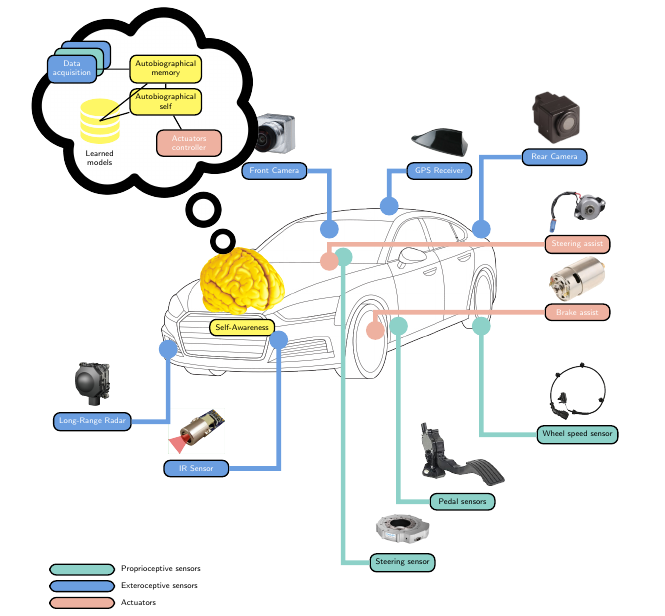
\includegraphics[scale=0.3]{regazzoni-2020-multi-sensorial-generative-and-descriptive-self-awareness-models-for-autonomous-systems-fig-1.png}
		\caption{See \cite{regazzoni-2020-multi-sensorial-generative-and-descriptive-self-awareness-models-for-autonomous-systems}}
	\end{figure}
\end{frame}

\begin{frame}{Damasio - Dispositional units}
	\begin{itemize}
		\item Lets make the contextually put together proprioceptive and extroceptive data over the course of time in two ways:
			\begin{itemize}
				\item Passive: An extroceptive piece of data is surrounded by two proprioceptive pieces of data
				\item Active: A proprioceptive piece of data is surrounded by two extroceptive piece of data 
			\end{itemize}
	\end{itemize}
	\begin{figure}
		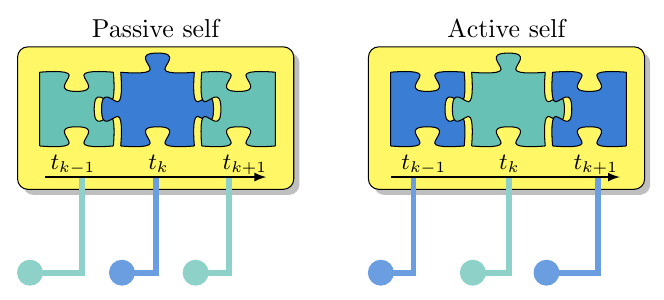
\includegraphics[scale=0.3]{regazzoni-2020-multi-sensorial-generative-and-descriptive-self-awareness-models-for-autonomous-systems-fig-2.png}
		\caption{See \cite{regazzoni-2020-multi-sensorial-generative-and-descriptive-self-awareness-models-for-autonomous-systems}}
	\end{figure}
\end{frame}

\begin{frame}{Damasio - HDU}
	\textbf{Hierarchical Dispositional Units (HDU)}
	\begin{itemize}
		\item To extract casual-temporal inferences, similar to brain, dispositionl units are contextually placed in one another in a hierarchy.
	\end{itemize}
	\begin{figure}
		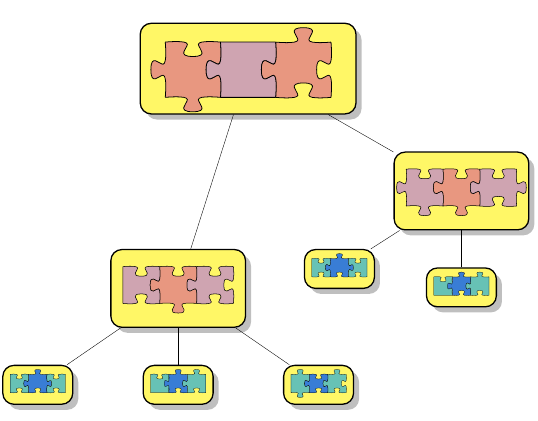
\includegraphics[scale=0.3]{regazzoni-2020-multi-sensorial-generative-and-descriptive-self-awareness-models-for-autonomous-systems-fig-3.png}
		\caption{See \cite{regazzoni-2020-multi-sensorial-generative-and-descriptive-self-awareness-models-for-autonomous-systems}}
	\end{figure}
\end{frame}

\begin{frame}{Damasio - AM}
	\textbf{Autobiographical Memory (AM)}
	\begin{itemize}
		\item Each set of dispositional units which contribute to building an experience is stored as an episode
		\item The collection of all episode forms the architecture of memory in the form a book which each page presents an episode. 
	\end{itemize}
\end{frame}

\begin{frame}{Damasio - AM}
	\begin{figure}
		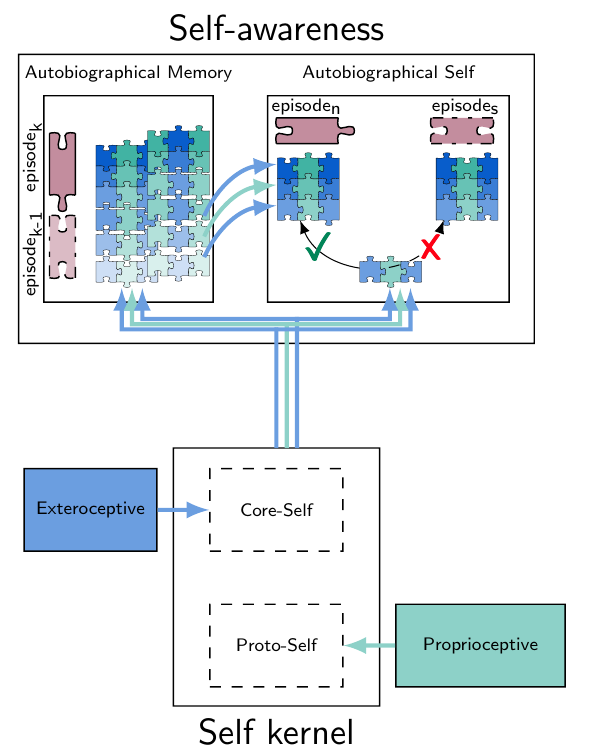
\includegraphics[scale=0.3]{regazzoni-2020-multi-sensorial-generative-and-descriptive-self-awareness-models-for-autonomous-systems-fig-4.png}
		\caption{See \cite{regazzoni-2020-multi-sensorial-generative-and-descriptive-self-awareness-models-for-autonomous-systems}}
	\end{figure}
\end{frame}

\begin{frame}{Damasio - Abnormality}
	\begin{itemize}
		\item Lets open the system's memory to observation through the time.
		\item Try to find a match for the set of observations in all AM pages with some acceptable noise tolerance (Most models use Hellinger metric to measure the distance between model's prediction and the set of observations)
			\begin{itemize}
				\item If there is a prediction(model/episode in AM) that falls bellow the tolerance for that set of observations then activate actuators as the models says. 
				\item If none of the predictions doesn't fall bellow the tolerance then its time to add a new episode (i.e page) to AM.
			\end{itemize} 
	\end{itemize}
	So another definition of self awareness is:
	\begin{itemize}
		\item Learning from large abnormalities
	\end{itemize}	
\end{frame}

\begin{frame}{Damasio - Abnormality}
	\begin{figure}
		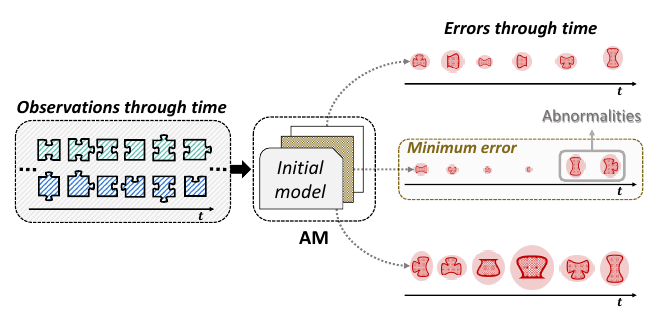
\includegraphics[scale=0.3]{regazzoni-2020-multi-sensorial-generative-and-descriptive-self-awareness-models-for-autonomous-systems-fig-8.png}
		\caption{See \cite{regazzoni-2020-multi-sensorial-generative-and-descriptive-self-awareness-models-for-autonomous-systems}}
	\end{figure}
\end{frame}


\begin{frame}{Computational SA approaches}
	\begin{itemize}
		\item Bayesian Model (BM): To model causality 
		\item Dynamic BM (DBM): To add temporality to causality model 
		\item Coupled DBM (To model dependence between Extroceptive and Proproceptive events)
		\item Generalized filtering (A non-linear space state Bayesian filtering) (To predict future state of an agent)
	\end{itemize}
\end{frame}

\begin{frame}{Collective SA (CA)}
	\textbf{Examples}:
	\begin{itemize}
		\item Bee colony
		\item Ant colony
		\item human imune system
	\end{itemize}
	In all above models no individual agent shares all the information with other agents but through development of a local interaction self-awareness which is distributed among all. Ants use pheromone samples left by other ants to locate the food. \textbf{Hence collective self-awareness is always decentralized and distributed.}  \cite{mitchell-2005-self-awareness-and-control-in-decentralized-systems}
\end{frame}

\begin{frame}{Computational CA application}
	\textbf{Examples}:
	\begin{itemize}
		\item Agent collision avoidance
		\item Traffic jam avoidance
	\end{itemize}
	\textbf{Benefits}:
	\begin{itemize}
		\item Improves scalability
		\item Reduces computational complexity through local-symbolic interaction
		\item Addresses heterogeneity by creating semantic fields
	\end{itemize}
\end{frame}

\begin{frame}{Computational CA approaches}
	See \cite{regazzoni-2020-multi-sensorial-generative-and-descriptive-self-awareness-models-for-autonomous-systems,kanapram-2020-collective-awareness-for-abnormality-detection-in-connected-autonomous-vehicles,kanapram-2019-self-awareness-in-intelligent-vehicles-experience-based-abnormality-detection}
	\begin{itemize}
		\item Lets correlate sets of observations of each agent with its true status
		\item Lets cluster the space of those states such that addition and removal of classes is possible during the time the procedure is taking place (Using Growing Gas Neural Networks (GGN)) - K-means and Self-organizing map doesn't help in this case.
		\item Use the attained clusters as letters of words to make the state space discreet.  
		\item Propagate the discreet states between the agents instead of real-data.
		\item Hellinger distance for abnormality detection
		\item Generate new models from large abnormalities.
	\end{itemize}
\end{frame}

\begin{frame}{References}
	\printbibliography
\end{frame}
\end{document}
